%!TEX root = ../../master.tex
\section{Experiment 2 - Resilience}
The following experiments are designed to accentuate ways of achieving better resilience in systems, especially systems consisting of microservices. As described in the chapter X\footnote{FIX ME: Insert reference}, we outline methods to achieve resilience as application level resilience and infrastructure level resilience. The experiments  serve the purpose of bridging the understanding for the students from Experiment 1, but they also serve the purpose of documenting the effects of different techniques to achieve application and infrastructure level resilience. \\
\noindent All tests in this section is performed using a load testing tool, Vegeta\footnote{FIX! Insert reference}. Vegeta is a versatile HTTP load testing tool that is able to apply load on a HTTP service with a constant request rate, making it ideal for testing the level of resilience in the following experiments.

\subsection*{Experiment 2.1 - Application level}
Application level refers to methods that can be applied by the developer to achieve a higher degree of resilience. The experiments described in this section will focus on the integration point in a synchronous architecture, and the derived anti-patterns and patterns that then can be applied.

\label{sec:experiment_application_level}
\subsubsection*{Experiment 2.1.1 - Integration points in a synchronous architecture} 
Integration points in a synchronous architecture must be handled with care. Nygard describes integration points as "[...] the number-one killer of systems"\cite[p. 46]{nygard2007release}, and he points out that this is where timeouts and circuit breakers come into play\footnote{Chapter 6}. These patterns are described by Nygard, but it has not been possible to find any data on the effects of them. \\
This experiment illustrates and documents the effects of circuit breakers when a service is unresponsive. \\

\noindent The test setup consists of three services running in a Kubernetes cluster. The three services form a chain in which Service 0 requests resources from Service 1 through HTTP, and Service 1 requests resources from Service 2 also through HTTP. A delay at 15 seconds is introduced in Service 2 to simulate an unresponsive and strained service. The services are implemented in Spring Boot using Netflix's circuit breaker called Hystrix. Further details can be found in Appendix C\footnote{FIX: MAKE SURE}. This exercises will investigate three scenarios that handle the delay at different degrees. The tests are executed from a computer running an HTTP load testing tool called Vegeta which makes requests on Service 0 through a cabled network. The scenarios are the following. \\

\noindent
\textit{1: No circuit breakers}
\\
In the first scenario, all requests between the services are synchronous calls without timeouts or circuit breakers (Figure~\ref{fig:exp2_no_circuit_breaker}). The expected result is that requests will pile up between Service 1 and Service 2 because of slow responses leading to blocked threads. The blocked threads should lead to a cascading failure making Service 1 unavailable and, at some point, Service 0 unavailable.

\begin{figure}[H]
\centering
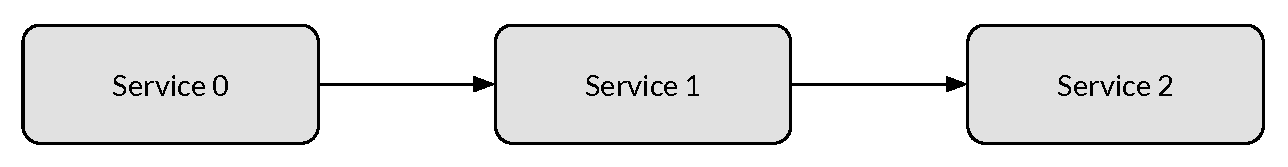
\includegraphics[scale=0.5]{figures/no_circuit_breaker_3_services}
\caption{Services without circuit breakers}
\label{fig:exp2_no_circuit_breaker}
\end{figure}

\noindent
\textit{2: One circuit breaker}
\\
In the second scenario, a timeout and circuit breaker is placed between Service 1 and Service 2 (Figure~\ref{fig:exp2_one_circuit_breaker}). The expected result is that the overall response time will improve since Service 1's timeout at 1 second decreases the time spent in blocked threads. Furthermore, the circuit breaker shuts off Service 2 at some point because of its slow responses.
\begin{figure}[H]
\centering
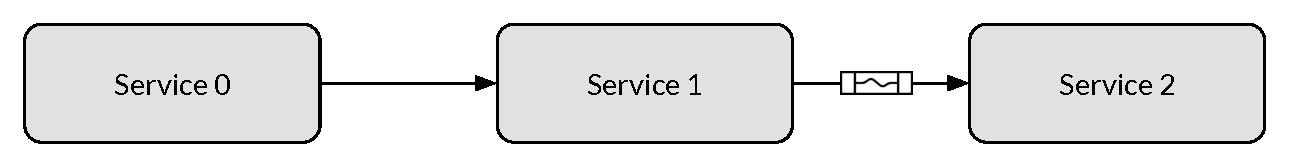
\includegraphics[scale=0.5]{figures/one_circuit_breaker_3_services}
\caption{Services with one circuit breaker}
\label{fig:exp2_one_circuit_breaker}
\end{figure}

\noindent
\textit{3: Two circuit breakers}
\\
In the third scenario, a circuit breaker is added between Service 0 and Service 1 and between Service 1 and Service 2 (Figure~\ref{fig:exp2_circuit_breaker}). This should lead to a latency below and at times up to the timeout between Service 0 and Service 1.
\begin{figure}[H]
\centering
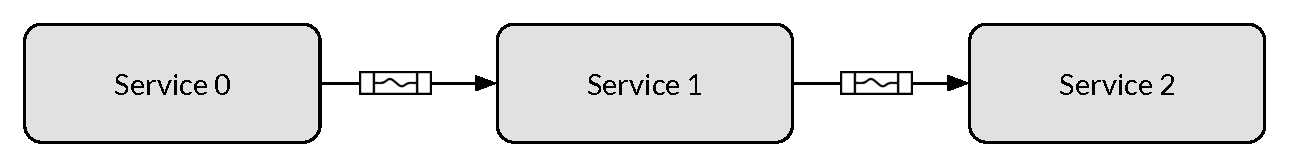
\includegraphics[scale=0.5]{figures/circuit_breaker_3_services}
\caption{Services with circuit breakers}
\label{fig:exp2_circuit_breaker}
\end{figure}

\noindent 

\noindent The expected result is that more circuit breakers lead to lower latencies and a higher success rate for requests. The results are expected to be degraded in the form of more fallback answers from Service 0 and Service 1. \\

\noindent Without circuit breakers the requests are expected to block all threads because of Service 2's delay cascading blocked threads while more requests are piling up. \\

\noindent When applying a circuit breaker in Service 1, towards service 2, the latencies are expected to be lower than without circuit breakers because Service 1 fails fast - the timeout is set to 1000ms. \\

\noindent With two circuit breakers the lowest latency is expected since the test runner's requests are directed towards Service 0 who's timeout is set to 1000ms. If the circuit breaker can follow up with the request rate, then the latency should not exceed 1000ms much. Another interesting aspect is the amount of fallback responses from Service 0 and Service 1. \\

\noindent
\textbf{Test protocol}
\\
For each iteration in each experiment the same state must be created. In order to do so a single instance of each service is started, which in Kubernetes terms is a deployment with a single pod with an exposed service in front of it. When all three services have started up, two requests to Service 0 is made with 10 seconds distance. This will ensure that all services are ready, and that the circuit breakers, if present, are in the \textit{closed} state. \\
After 15 seconds, which is the duration of the delay in Service 2, the test runner can be started. The test runner generate 100 requests/second for 30 seconds which leads to 3000 measurements.\\

\noindent
When the test runner has finished its run, the Kubernetes pods are deleted and fresh instances created. The test protocol steps can then be repeated.\\

\noindent
\textbf{Metrics} \\
The main metrics resulting from the experiments are \textit{latency}, \textit{success rate} and \textit{level of demotion}.\\

\noindent
The latency is a value between 0s and 30s since the test runner's timeout is set to 30s. The success rate is based on the HTTP status codes returned. 200 denotes a success and 206 denotes a success from a circuit breaker. The level of demotion is measured as the distribution of the responses' origins. A response from service 2 is the desired and best response. Subsequently Service 1 is preferred over Service 0. \\

\noindent FIX: Pool size initially 3, up to 10 (maybe here, maybe in discussion?)
\\ What type of thread pool? Are hanging threads being preempted? \\

\noindent
\textbf{Data basis}
\\
Three iteration of each scenario is run to reduce the impact of random factors. In each iteration 3000 measurements will be made which sums up to 9000 measurements per scenario.

%\subsubsection*{Experiment 2.1.2 - Latency injection} 
%
%\textbf{Test protocol}
%\textbf{Metrics}
%Latency, success rate, content
%\textbf{Data basis}

\subsection*{Experiment 2.2 - Infrastructure level}
\label{sec:experiment_infrastructure_level}
The previous section focused on the effects of application level patterns to achieve a higher degree of resilience. This section will instead look into designing experiments to verify the different initiatives possible at the infrastructure level. Fault tolerance and the ability to detect failures are among the most notable features to ensure a higher degree of resilience at the infrastructure level, as described in chapter X\footnote{FIX! REFERENCE TIL KAPITEL OM INFRASTUCTURE LEVEL RESILIENCE}.

\subsubsection*{Experiment 2.2.1 - The effects of replication}
\label{sec:experiment:effects_of_replication}
Fault tolerance is a key feature in Kubernetes. The goal of this experiment is to look into the effects of replication in order to determine the number of replicas needed in order to handle different amounts of load. \\ \\
\noindent The test setup consist of one simple application written in Java with the Spring Boot framework. The application is packaged into a Docker container and deployed into Kubernetes. The application is returning a string when it receives a HTTP request at '/'. This experiment will be doing ramp up, which referes to continuing to apply more and more load, to stress the system. The increase of request per second is being done with requesting 10.000 request at each step. The step size will be set to an increase at 100 request/second. Calculating the duration at each step is done using the following formula: \\

\[ duration_{step}
  = \dfrac{10.000 + (rate_{current}-1)}{rate_{current}}
\] \\

\noindent This experiment will be repeated with replicas=1, replicas=5, and replicas=10. Each experiment will de run 3 times, to eliminate randomness and the worst outliers. Average of the 3 runs will be applied. All load will be generated by a MacBook Pro and directed directly add the service endpoint '/'. \\ \\
\noindent The expected result is that replicating the application will result in a higher degree of resilience.\\

\noindent\textbf{Test protocol}\\
Every test shall be run with a 'clean' environment. The test protocol of this experiment is as follows:

\begin{enumerate}
  \item Run the application in Kubernetes (start the pod)
  \item Expose the application in Kubernetes (add a service)
  \item Scale the deployment to the desired number of replicas
  \item Start the test script in section X\footnote{FIX! Find ud af hvordan man laver referencer til lstlisting}
\end{enumerate}

\noindent Steps 1-4 shall be run in total of three times.\\


\noindent\textbf{Metrics}\\
The main metric in this experiment is \textit{latency}, and especially the point at which the latency will have an exponential increase. \\

\noindent\textbf{Data basis}\\
Three iteration of each experiment is run to reduce the impact of random factors.

\subsubsection*{Experiment 2.2.2 - Recovery time} 
\label{sec:experiment:recovery}
Another key feature of Kubernetes as a platform is the ability to detect failures, e.g. that the container has crashed or that the node has been removed from the cluster. The goal of this experiment is to look into this ability and try to determine the recovery time of an application, by only deploying one instance of the application. The second part of this experiment is to verify that by increasing the number of replicas the infrastructure will be able to handle a node failure with a minimum of lost requests. \\ 

\noindent The test setup consist of the same application used in the previous experiment (section \ref{sec:experiment:effects_of_replication}). Since the goal of this experiment is to determine the effects of losing af node, we will pull the network cable of a node running the application (pod). The experiment will be running with a total duration of 3 minutes (180 seconds) for each iteration, and the network cable will be removed after 30 seconds. The experiment will be run with replicas=1, replicas=2, and replicas=5 and with rate=100 request/second, and rate=200 request/second.\\

\noindent The expected result is that with only one replication the application will be unresponsive for about 5 seconds (--pod-eviction-timeout) + 10 seconds (--node-grace-period) + 25 seconds (Spring Boot boot time on the Raspberry Pi) = 40 seconds. Whereas the expected result for running more than one replica will result in a significant lower amount of lost request.

\noindent\textbf{Test protocol}\\
Every iteration of test has to be run with a 'clean' environment. The test protocol is as follows:
\begin{enumerate}
  \item Run the application in Kubernetes (start the pod)
  \item Expose the application in Kubernetes (add a service)
  \item Scale the deployment to the desired number of replicas
  \item Determine where the application (pod) has been started
  \item Start a stopwatch and test script at the same time
  \item After 30 seconds, remove the network cable of the node where the pod is running
\end{enumerate}
\noindent Steps 1-6 shall be run in total of three times. If the application is scheduled on the master node, it is necessary to delete the pod and start it again to be rescheduled on a slave node. We only pull the plug of nodes with one application (pod) running.\\

\noindent\textbf{Metrics}\\
The two main metrics in this experiment are \textit{the recovery time in seconds} and the \textit{success rate in percent}.\\

\noindent\textbf{Data basis}\\
Three iteration of each experiment is run to reduce the impact of random factors.
